\documentclass{article}

\usepackage{fullpage}
\usepackage{graphicx}


\title{Práctica 6: Filtros activos}
\date{}
\author{Pablo Cuesta Sierra. Grupo 1201.}



\begin{document}

\maketitle
\begin{center}
\section{TRABAJO PREVIO (Simulación LTSpice y cálculos teóricos)}
\end{center}
\paragraph{a. Dibuje el circuito 1 con los valores de componentes mostrados en la figura. Use el modelo de  Amplificador  Operacional  Universal  (UniversalOpamp2) dentro  de  la  carpeta  [Opamps] Vcc=12V  y  Vee=-12V  son  las  tensiones  de  alimentación  simétricas  para  el  Amplificador Operacional.}

\paragraph{b. Conecte una fuente de tensión a la entrada Vin de tipo sinusoidal de frecuencia y amplitud arbitraria. Asegúrese  de  que  la  amplitud  en  la  señal  de  entrada  no  alcanza  las  tensiones  de saturación del amplificador operacional a la salida.\\}

Como se calcula en \textbf{(c)}, la ganancia es de valor $2=|\frac{V_{out}}{V_{in}}|$, por lo que para no alcanzar las tensiones de saturación, basta con tomar $V_{in}<6V$, para simplificar, tomaré amplitud $1V$, además de una frecuencia de 100Hz (he incluido el comando de la simulación, para ver las señales en un tiempo de 30ms):
\bigskip
\begin{center}
\centerline{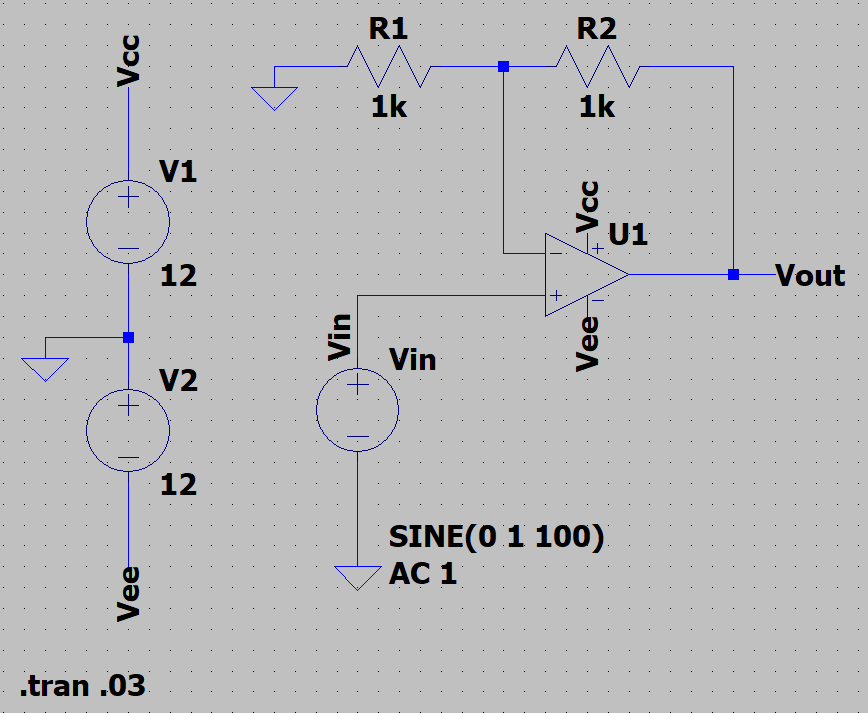
\includegraphics[scale=0.5]{c1lts}}
{Dibujo Circuito 1 en LTSpice.}
\label{fig1}
\end{center}
\cleardoublepage

\paragraph{c. Determine la ganancia del amplificador y el desfase entre la señal de entrada y la de salida. Compare la ganancia simulada con la calculada teóricamente.\\}



Cálculos teóricos:

\centerline{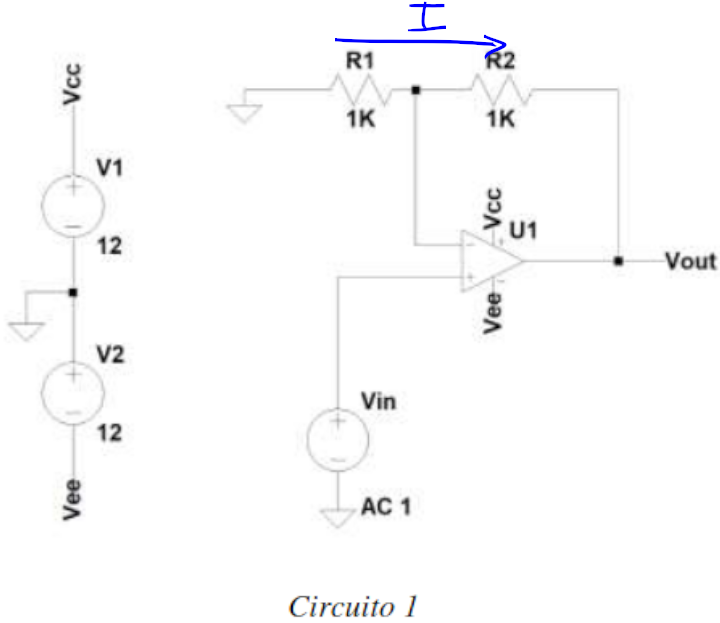
\includegraphics[scale=0.3]{c1}}

Como el AO está realimentado negativamente, asumimos que $v^+=v^-=v_{in}$. 
$$\Rightarrow I=\frac{0-v_{in}}{R_1}=\frac{v_{in}-v_{out}}{R_2}\Rightarrow v_{out}=R_2 v_{in} \left( \frac{1}{R_1}+\frac{1}{R_2}\right)=2\ v_{in}\Rightarrow A_v=\frac{v_{out}}{v_{in}}=2.\ \ |A_v|=2.\ \ \phi_{A_v}=0$$

En la simulación, como está configurada en la imagen del apartado anterior:
\begin{center}
\centerline{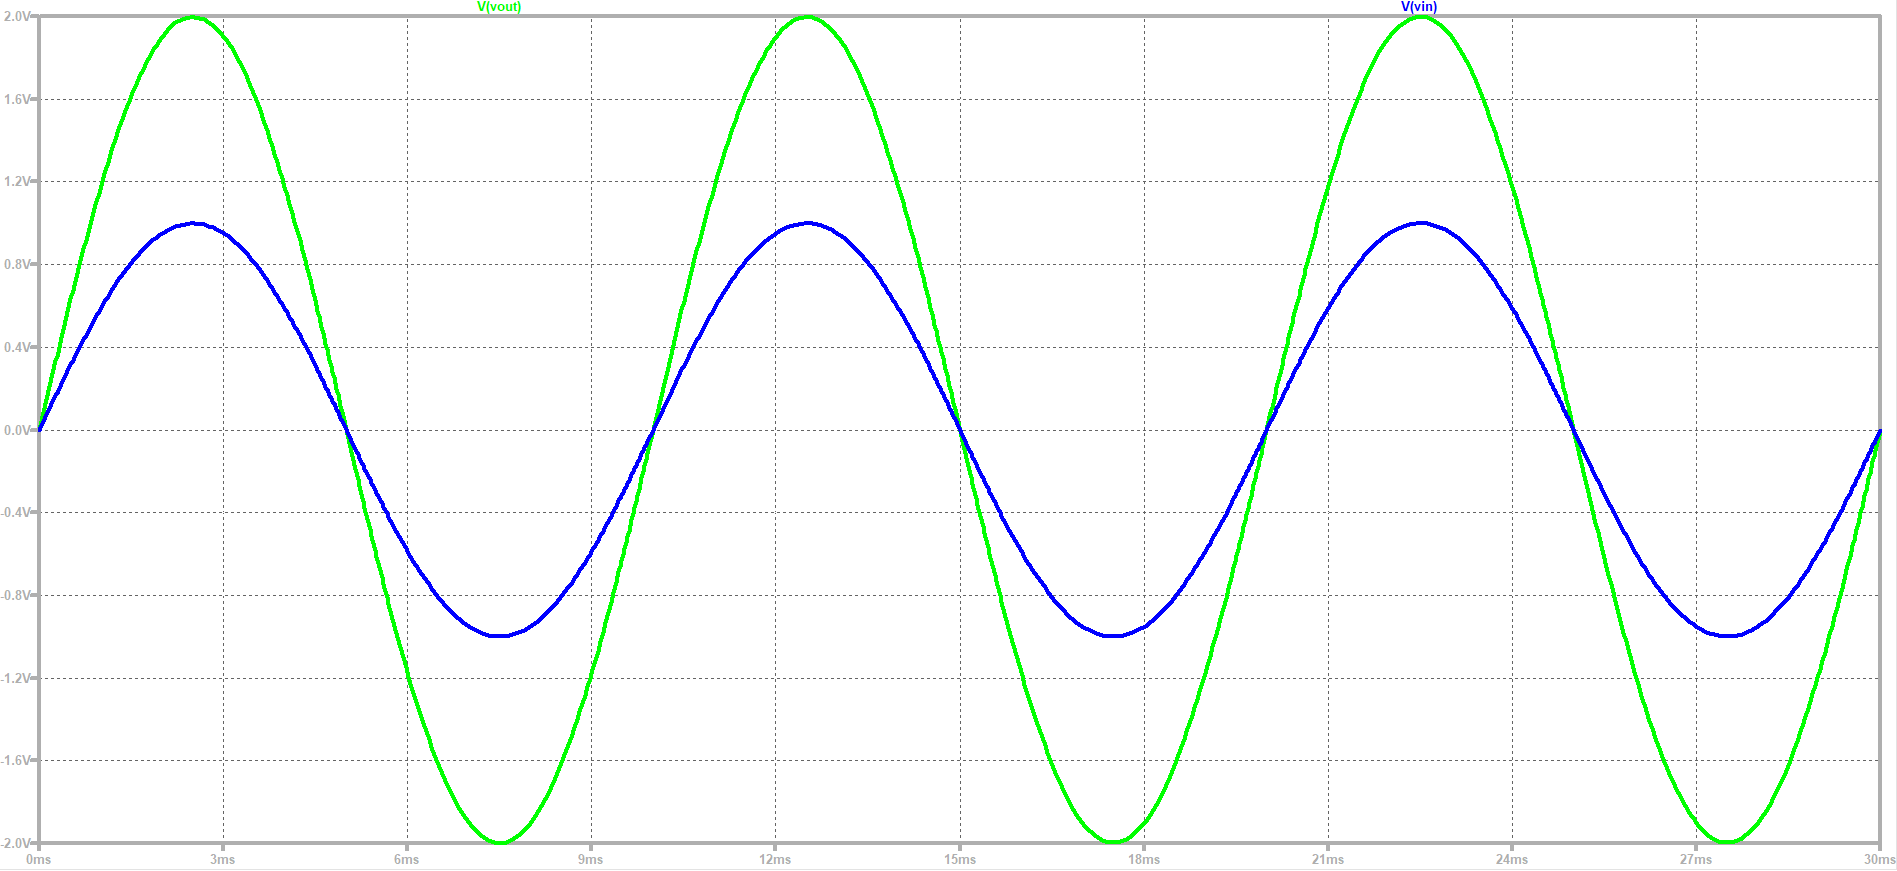
\includegraphics[scale=0.3]{c1dem}}

$V_{out}$, en verde. $V_{in}$, en azul.
\end{center}
Podemos comprobar que la diferencia de fase es nula y que la amplitud de $V_{out}$ es 2V, el doble que la de $V_{in}$.

\begin{center}
\centerline{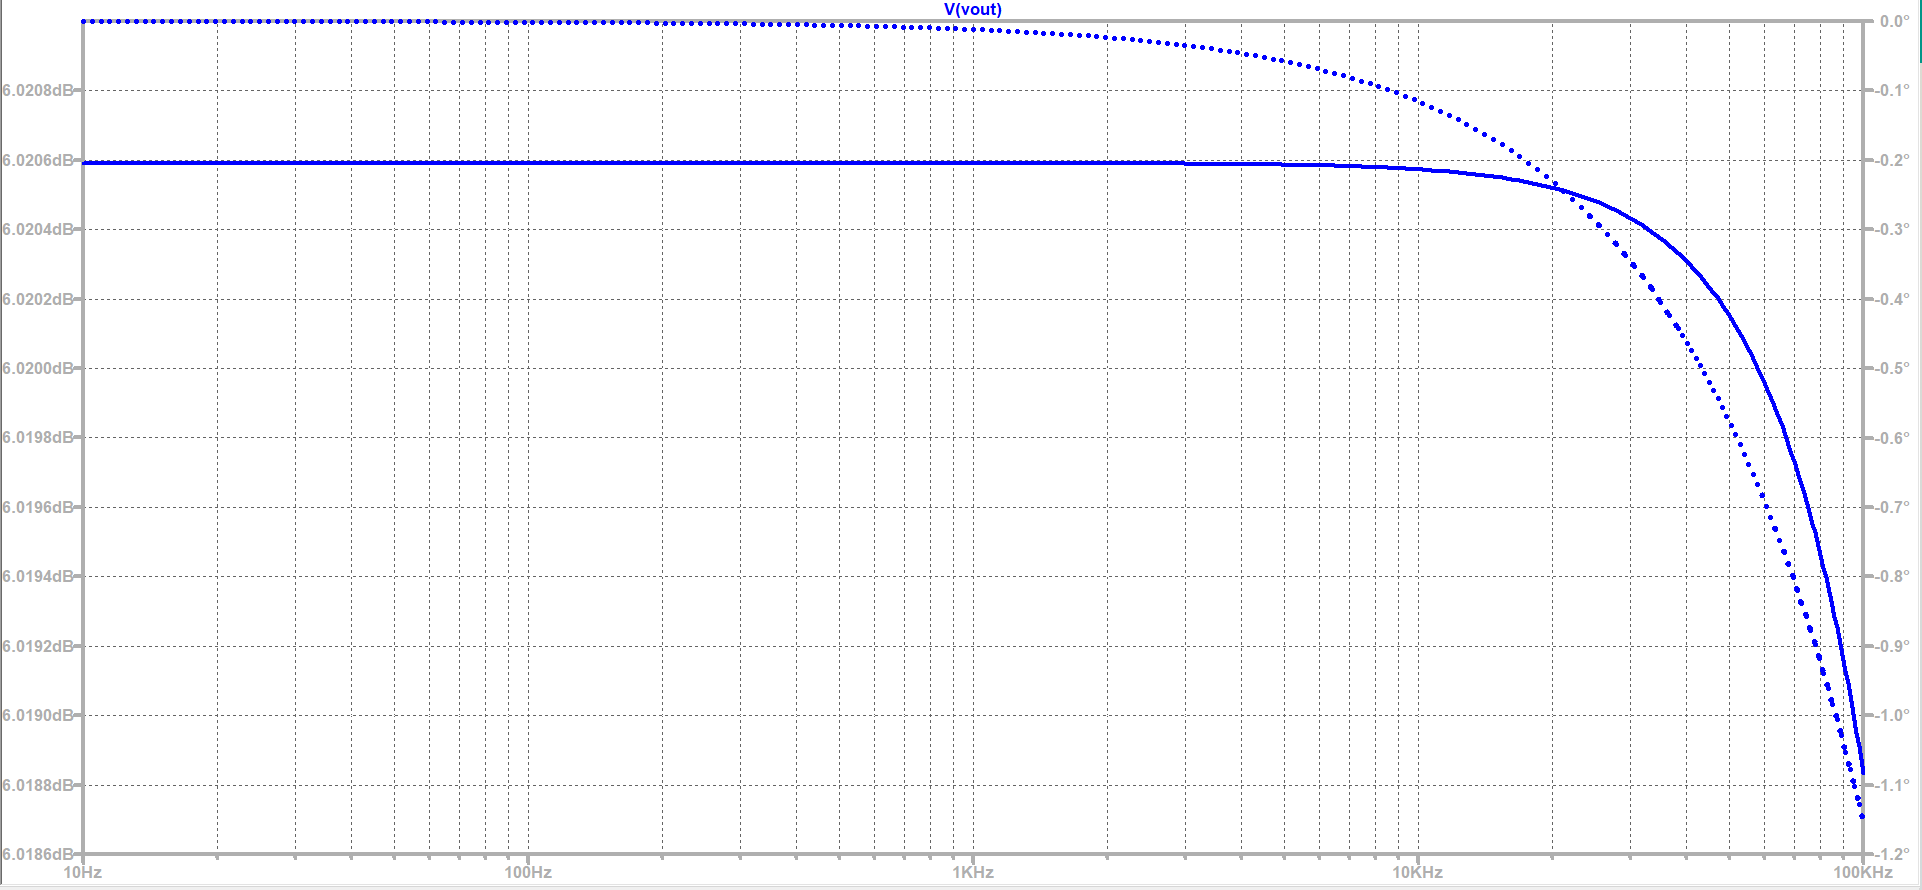
\includegraphics[scale=0.4]{apart_c}}
Barrido de frecuencias en alterna. Vout representa la ganancia, ya que la señal de entrada tiene 1V de amplitud. 
\end{center}
Se ha utilizado el comando:
\begin{verbatim}
	.ac dec 101 10 100000
\end{verbatim}

Se puede ver que la ganancia es constante en los valores hasta 100kHz, con un valor de $20\log_{10}{2}\approx 6,0206dB$, como era de esperar, y para estas frecuencias la fase se mantien constante en 0$^o$. Sin embargo, se observa que para las frecuencias más altas, la ganancia empieza a caer ligermante y comienza a haber una diferencia de fase, aunque pequeña. 

Esto se puede deber al delay que tiene el amplificador operacional (lo que terda en transmitirse la corriente desde que entra hasta que sale), que con frecuencias tan altas, comienza a producirse un desfase entre su entrada y su salida que se muestra de esta forma en la gráfica de la simulación.
\cleardoublepage

\paragraph{d. Conecte un filtro RC a la entrada no inversora del Amplificador Operacional siguiendo el
esquema del circuito 2. Conecte a la entrada del filtro una fuente de tensión alterna V3 de
amplitud 1 V.\\}

\begin{center}
\centerline{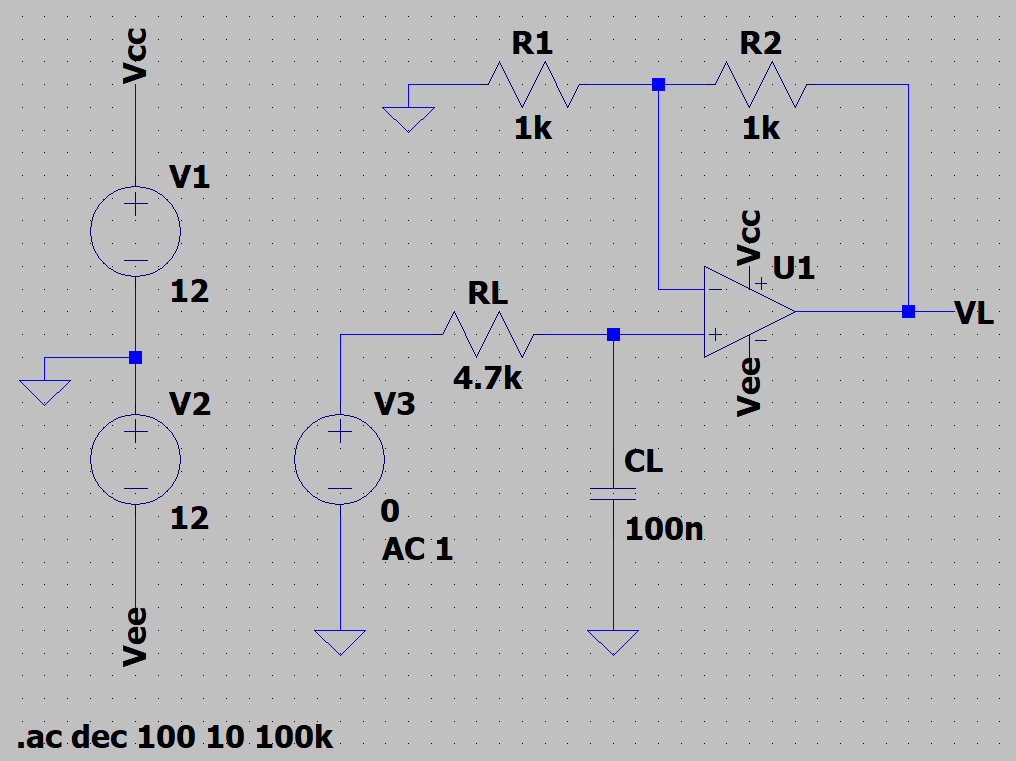
\includegraphics[scale=0.3]{c2dib}}

Dibujo Circuito 2 en LTSpice.
\end{center}

\paragraph{e. Mediante una simulación en alterna determine el comportamiento del circuito con la
frecuencia de V3. Dibuje la ganancia VL/V3 y el desfase entre las dos señales en función de la
frecuencia en el rango 10 Hz - 100 KHz.\\}

\begin{center}
\centerline{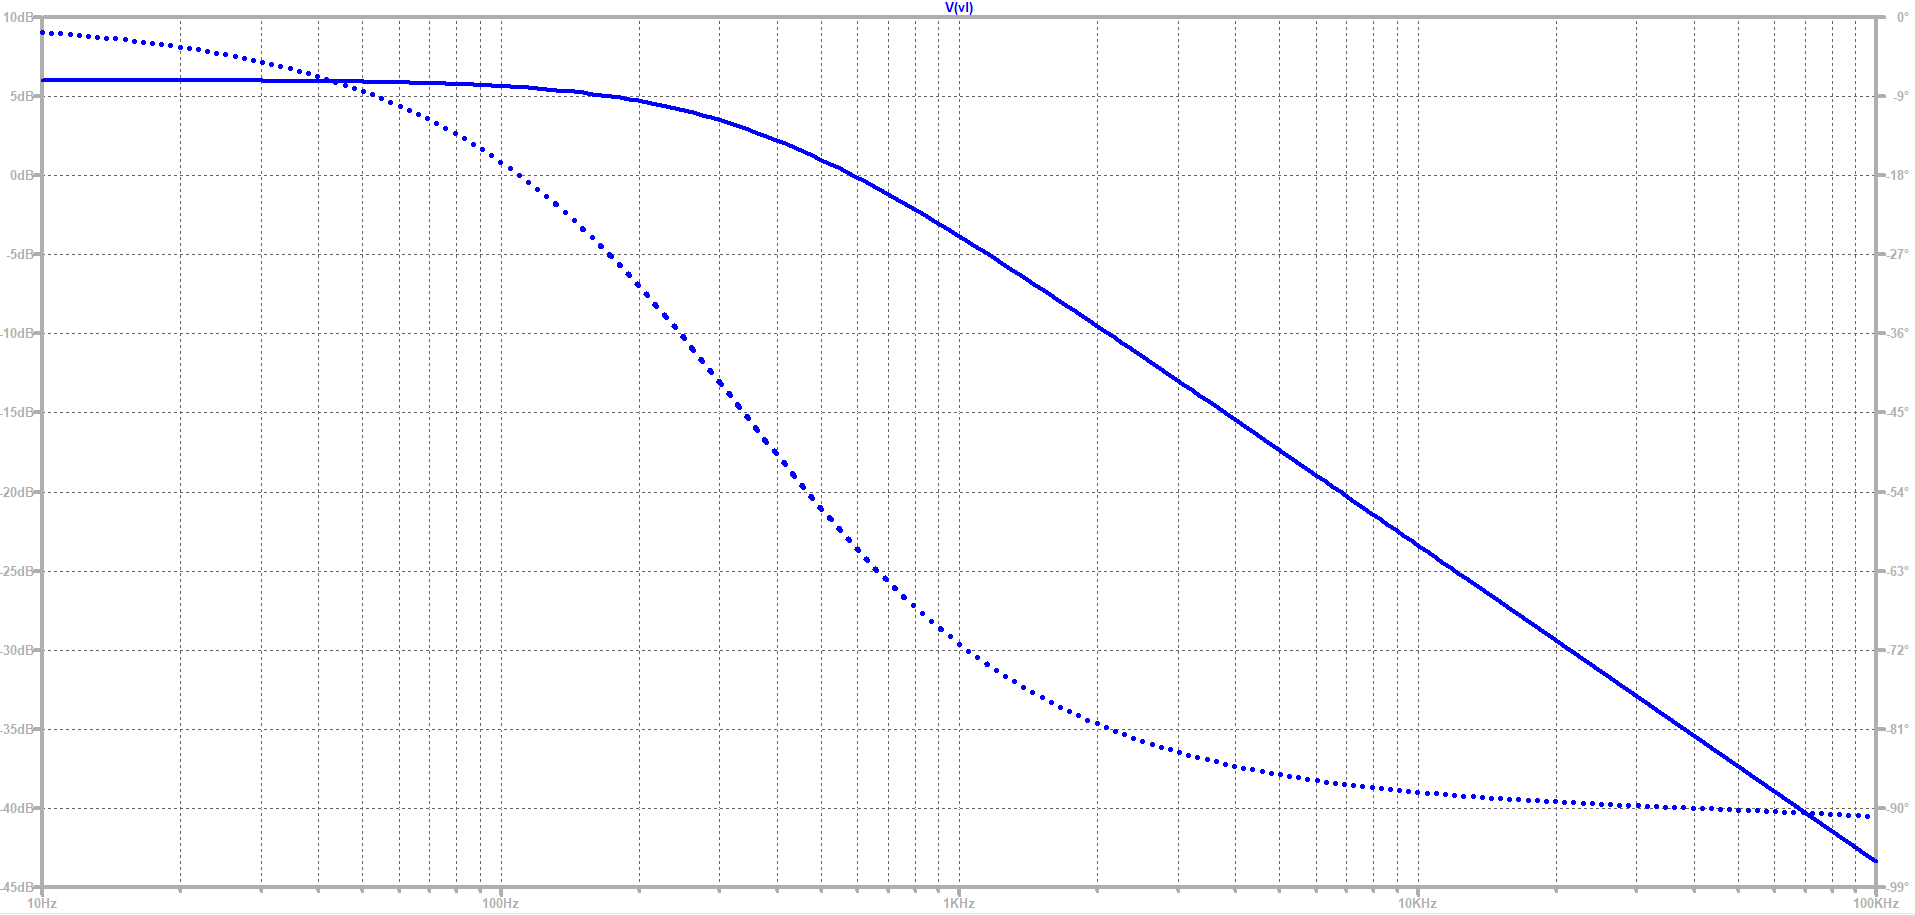
\includegraphics[scale=0.3]{c2dem}}

Gráfica de $A_v$ (ya que $|V_3|=1V$), tanto la fase (puntos discontinuos) como la norma. Representada frente a la frecuencia.
\end{center}

\paragraph{f. ¿Qué tipo de filtrado que realiza el circuito sobre la señal de entrada: paso alto, paso bajo o
paso banda? Determine la frecuencia o frecuencias de corte a partir de la representación gráfica
de la simulación y mediante el cálculo teórico.\\}
Como se puede apreciar en la gráfica, corresponde a un filtro de paso bajo.

\cleardoublepage

Cálculos teóricos:

\centerline{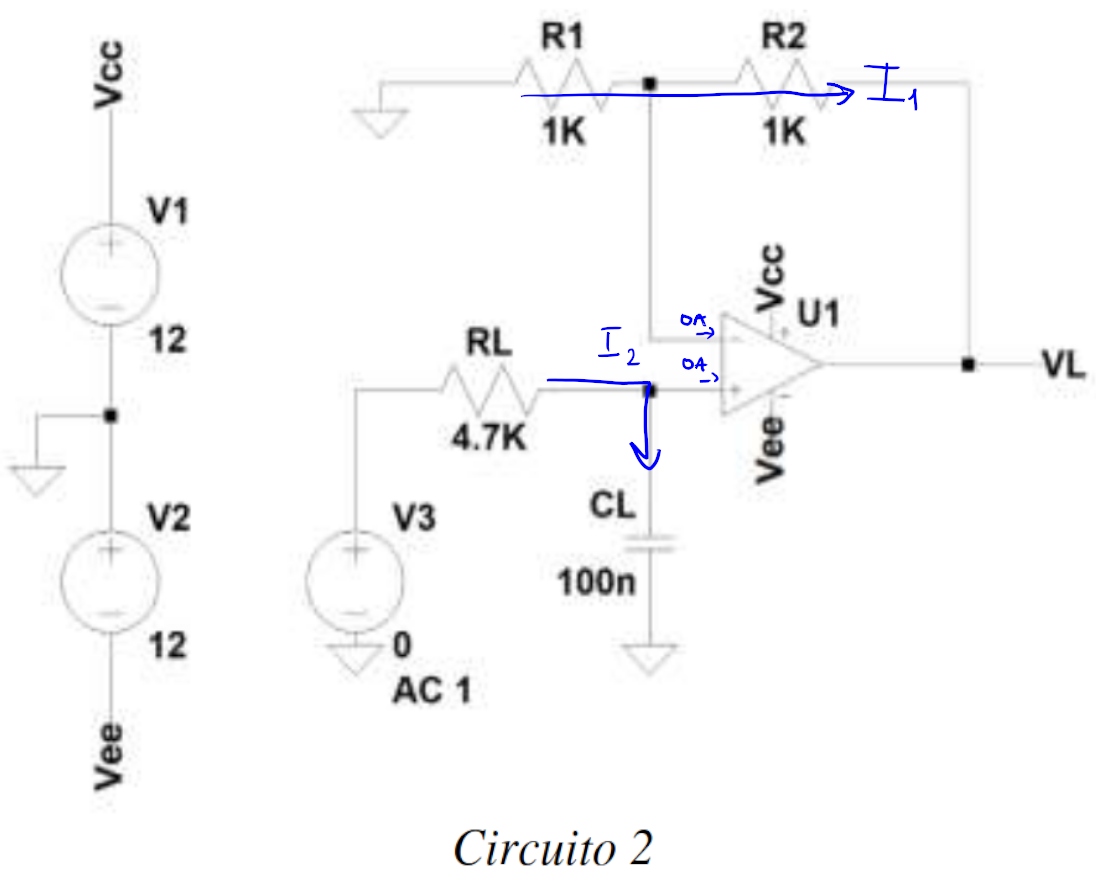
\includegraphics[scale=0.3]{c21}}

De nuevo, como el AO está realimentado negativamente, asumimos que $v^+=v^-$. Entonces, 

$$I_2=\frac{v_3-v^+}{R_L}=\frac{v^+}{Z_{C_L}}\Rightarrow v^+\left(\frac{1}{Z_{C_L}}+\frac{1}{R_L}\right)=\frac{v_3}{R_L}\Rightarrow v^+=\frac{v_3 Z_{C_L}}{R_L+Z_{C_L}}=\frac{v_3}{1+\frac{R_L}{ Z_{C_L}}}$$
Por otro lado,
$$I_1=\frac{0-v^-}{R_1}=\frac{v^--v_{L}}{R_2}\Rightarrow v_L=R_2 v^- \left( \frac{1}{R_1}+\frac{1}{R_2}\right)=2\ v^-= 2\ v^+ = \frac{2\ v_3}{1+\frac{R_L}{ Z_{C_L}}}$$

$$\Rightarrow A_v(jf)=\frac{v_L}{v_3}=\frac{2}{1+\frac{R_L}{ Z_{C_L}}}=\frac{2}{1+j2\pi f C_L R_L}$$ $$\Rightarrow |A_v|(f) = \frac{2}{\sqrt{1+(2\pi f C_L R_L)^2}}, \ \ \phi (f)=-\arctan{(2\pi f C_L R_L)}$$

El valor de la frecuencia de corte:

$$|A_v|^{max}=2=|A_v|(0)\Rightarrow |A_v|(f_c)=\frac{2}{\sqrt2}\iff f_c=\frac{1}{2\pi C_L R_L}\approx 338,628 Hz$$
además, $\phi(f)=-\arctan{(f/f_c)}\Rightarrow \phi(f_c)=-45^o$.

En la simulación, para obtener la frecuencia de corte, por tanto, tengo que mover el cursor hasta la frecuencia en la que la fase sea de valor -45$^o$:

\begin{center}
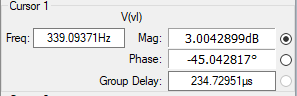
\includegraphics[scale=0.6]{145}
\end{center}

lo que nos da una frecuencia de corte en la simulación de 339,094Hz, por lo que se ha tenido un error de:
$E_r=100\times\frac{|339,094-338,628|}{339,094}=0,137\%$

\cleardoublepage
En la siguiente tabla utilizo estas fórmulas para unas pocas frecuencias:

\begin{table}[h]
\centering
\begin{tabular}{|r|r|r|r|}
\hline
\multicolumn{1}{|l|}{frecuencia (Hz)} & \multicolumn{1}{l|}{$|A_v|$} & \multicolumn{1}{l|}{$|A_v|(dB)$} & \multicolumn{1}{l|}{$\phi (f) (^o)$} \\ \hline
10                                    & 1,999128492                                       & 6,016814176                      & -1,691508405                         \\ \hline
100                                   & 1,91811089                                        & 5,65747422                       & -16,45238226                         \\ \hline
1000                                  & 0,6414744806                                      & -3,856412324                     & -71,29248409                         \\ \hline
10000                                 & 0,06768671111                                     & -23,38993175                     & -88,06054821                         \\ \hline
100000                                & 0,00677251194                                     & -43,38500441                     & -89,80598145                         \\ \hline
\end{tabular}
\end{table}


Los valores en la simulación para las mismas frecuencias:
\begin{center}
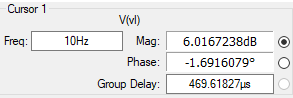
\includegraphics[scale=0.6]{110}
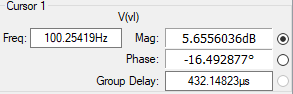
\includegraphics[scale=0.6]{1100}
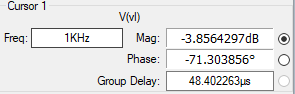
\includegraphics[scale=0.6]{11000}\\
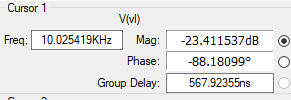
\includegraphics[scale=0.6]{110000}
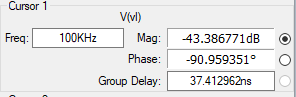
\includegraphics[scale=0.6]{1100000}
\end{center}

Que difieren muy ligeramente de los teóricos (porque en muchos casos no se podía poner el cursor exactamente en la frecuencia deseada).

\paragraph{g. Repita los apartados d) e) y f) para el circuito 3. En este circuito la red RC se ha sustituido por otra distinta (note que, además de intercambiar el condensador y la resistencia de posición, se ha reducido el valor del condensador de 100 nF a 10nF.}

\begin{center}
\centerline{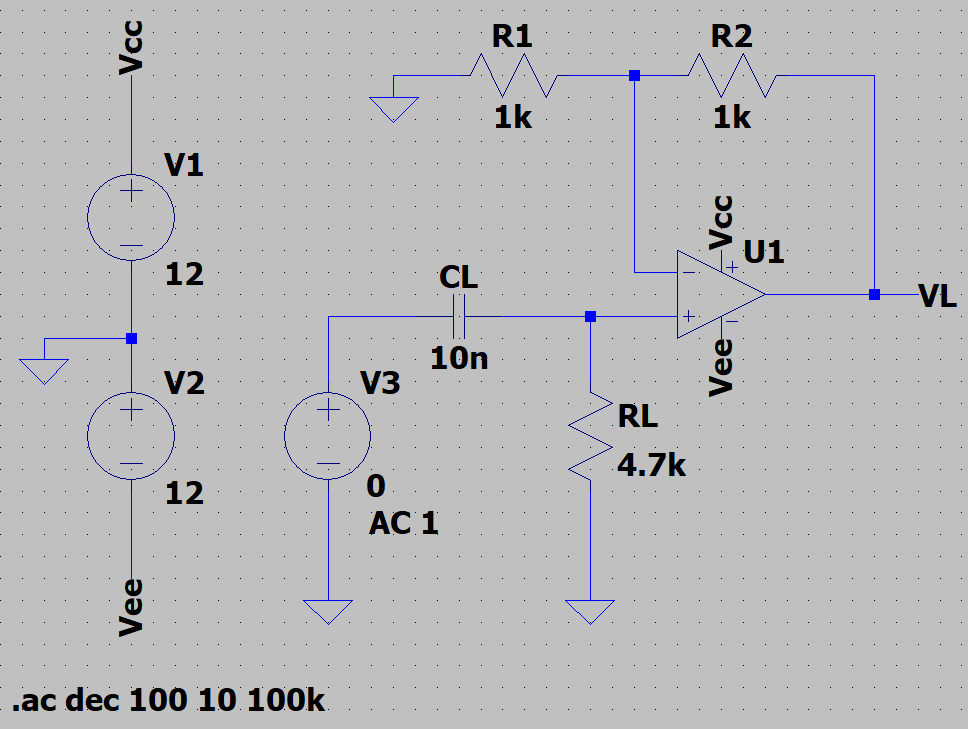
\includegraphics[scale=0.5]{c3dib}}

Dibujo Circuito 3 en LTSpice.
\end{center}
\begin{center}
\centerline{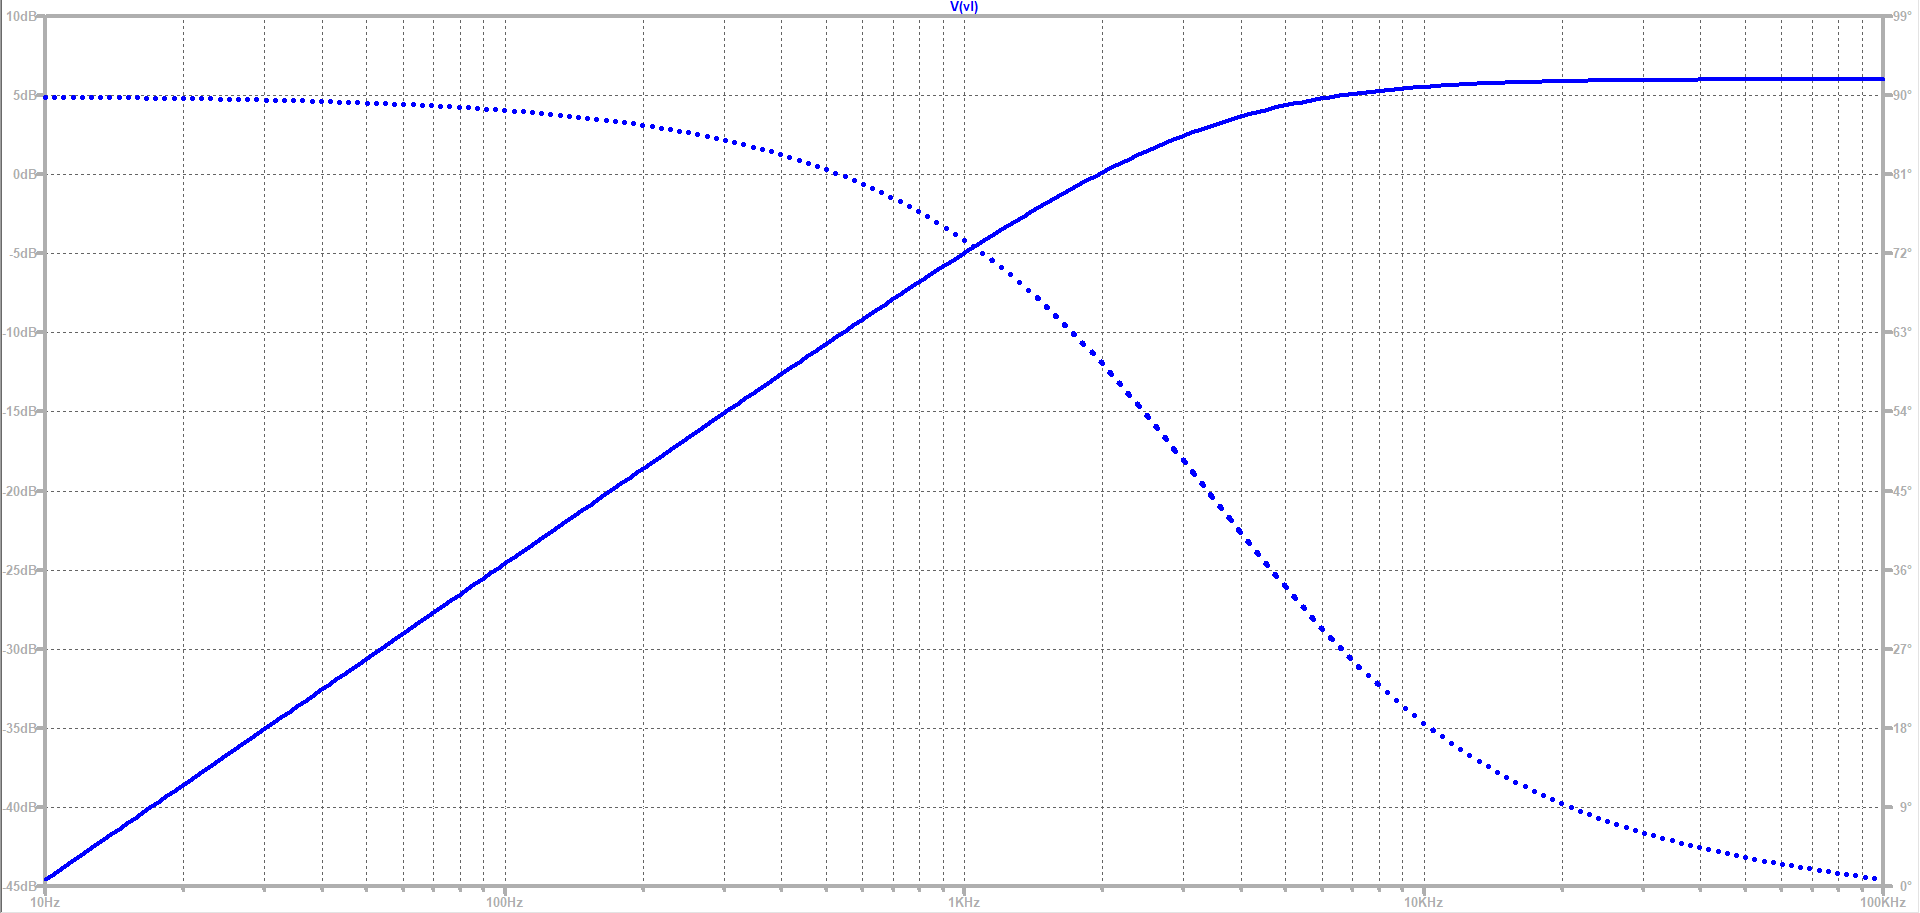
\includegraphics[scale=0.3]{c3dem}}

Gráfica de $A_v$ (ya que $|V_3|=1V$), tanto la fase (puntos discontinuos) como la norma. Representada frente a la frecuencia.
\end{center}

Este circuito corresponde a un filtro de paso alto.
    
Cálculos teóricos:

\centerline{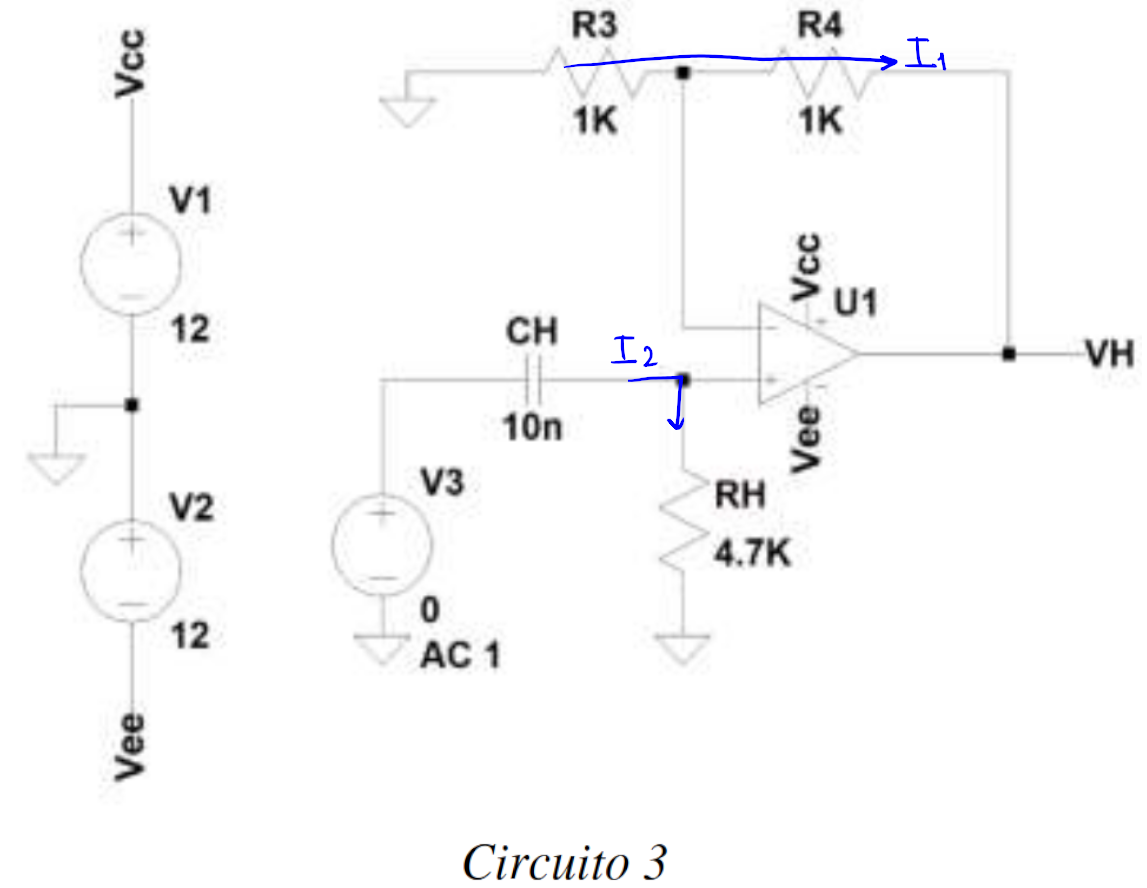
\includegraphics[scale=0.3]{c31}}

El AO está realimentado negativamente, por lo que asumimos que $v^+=v^-$. Entonces, como antes (los cálculos de $I_1$ no varían):
$$I_1=\frac{0-v^-}{R_1}=\frac{v^--v_{L}}{R_2}\Rightarrow v_L=R_2 v^- \left( \frac{1}{R_1}+\frac{1}{R_2}\right)=2\ v^-$$
$$I_2=\frac{v_3-v^+}{Z_{C_L}}=\frac{v^+}{R_L}\Rightarrow v^+\left(\frac{1}{Z_{C_L}}+\frac{1}{R_L}\right)=\frac{v_3}{Z_{C_L}}\Rightarrow v^+=\frac{v_3 R_L}{R_L+Z_{C_L}}=\frac{v_3}{1+\frac{Z_{C_L}}{R_L}}$$
Por tanto,
$$v_L=2\ v^-=2\ v^+=\frac{2\ v_3}{1+\frac{Z_{C_L}}{R_L}}=\frac{2\ v_3}{1-\frac{j}{2\pi f C_L R_L}}$$

$$A_v(jf)=\frac{v_L}{v_3}=\frac{2}{1-\frac{j}{2\pi f C_L R_L}}, \ \ |A_v|(f)=\frac{2}{\sqrt{1+\frac{1}{(2\pi f C_L R_L)^2}}}, \ \ \phi(f)=-\arctan{\left(\frac{-1}{(2\pi f C_L R_L)}\right)}$$

La frecuencia de corte (se calcula de la misma forma que en el Circuito 2, aunque cambia el valor porque el valor de $C_L$ es diferente):
$$|A_v|^{max}=2=|A_v|(0)\Rightarrow |A_v|(f_c)=\frac{2}{\sqrt2}\iff f_c=\frac{1}{2\pi C_L R_L}\approx 3386,275 Hz$$

De nuevo, con estas fórmulas he rellenado una tabla como la anterior:


\begin{table}[h]
\centering
\begin{tabular}{|r|r|r|r|}
\hline
\multicolumn{1}{|l|}{frecuencia (Hz)} & \multicolumn{1}{l|}{$|A_v|$} & \multicolumn{1}{l|}{$|A_v|(dB)$} & \multicolumn{1}{l|}{$\phi (f) (^o)$} \\ \hline
10                                    & 0,005906168436                                    & -44,57388343                     & 89,83080049                          \\ \hline
100                                   & 0,0590362054                                      & -24,5776313                      & 88,30849159                          \\ \hline
1000                                  & 0,5664367696                                      & -4,936971254                     & 73,54761774                          \\ \hline
10000                                 & 1,894336425                                       & 5,549142202                      & 18,70751591                          \\ \hline
100000                                & 1,998854299                                       & 6,015622772                      & 1,939451791                          \\ \hline
\end{tabular}
\end{table}


Los valores en la simulación para las mismas frecuencias:

\begin{center}
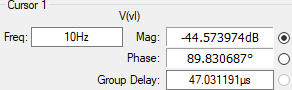
\includegraphics[scale=0.6]{210}
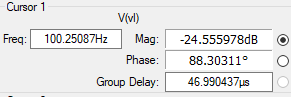
\includegraphics[scale=0.6]{2100}
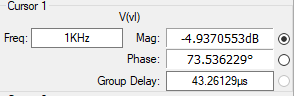
\includegraphics[scale=0.6]{21000}\\
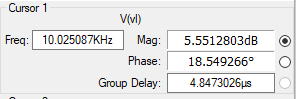
\includegraphics[scale=0.6]{210000}
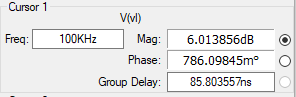
\includegraphics[scale=0.6]{2100000}
\end{center}

De nuevo, no hay diferencia entre los valores de la simulación y los obtenidos mediante los cálculos teóricos. (Las diferencias se deben a que no siempre se puede poner el cursor sobre la frecuencia deseada.)

En este caso, con la frecuencia de corte tenemos que $\phi (f)=-\arctan(-f_c/f)$, por tanto, $\phi (f_c)=+45^o$. Así que buscando en la gráfica de la simulación la frecuencia en la que la fase tiene este valor, hallamos:

\centerline{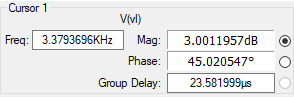
\includegraphics[scale=0.6]{245}}

Es decir, que la frecuencia de corte en la simulación corresponde a 3379,370Hz, es decir, tiene un error relativo con el valor teórico de 
$E_r=100\times\frac{|3379,370-3386,275|}{3379,370}=0,204\%$
\cleardoublepage

\begin{center}
\section{Montaje experimental}
\end{center}

\textbf{Construya en el panel de la entrenadora el circuito 2. Dicho circuito incluye un
amplificador no inversor como el analizado en el circuito 1 del Trabajo Previo. El Amplificador
Operacional se alimentará utilizando las fuentes S1 y S2 con tensiones de salida de 12 V y un
conexionado como el que muestra la foto.}

\textbf{La señal V3 de entrada a los circuitos la proporciona el generador de funciones. Fije una
tensión sinusoidal de amplitud 1V para la caracterización.}
\bigskip
\begin{center}
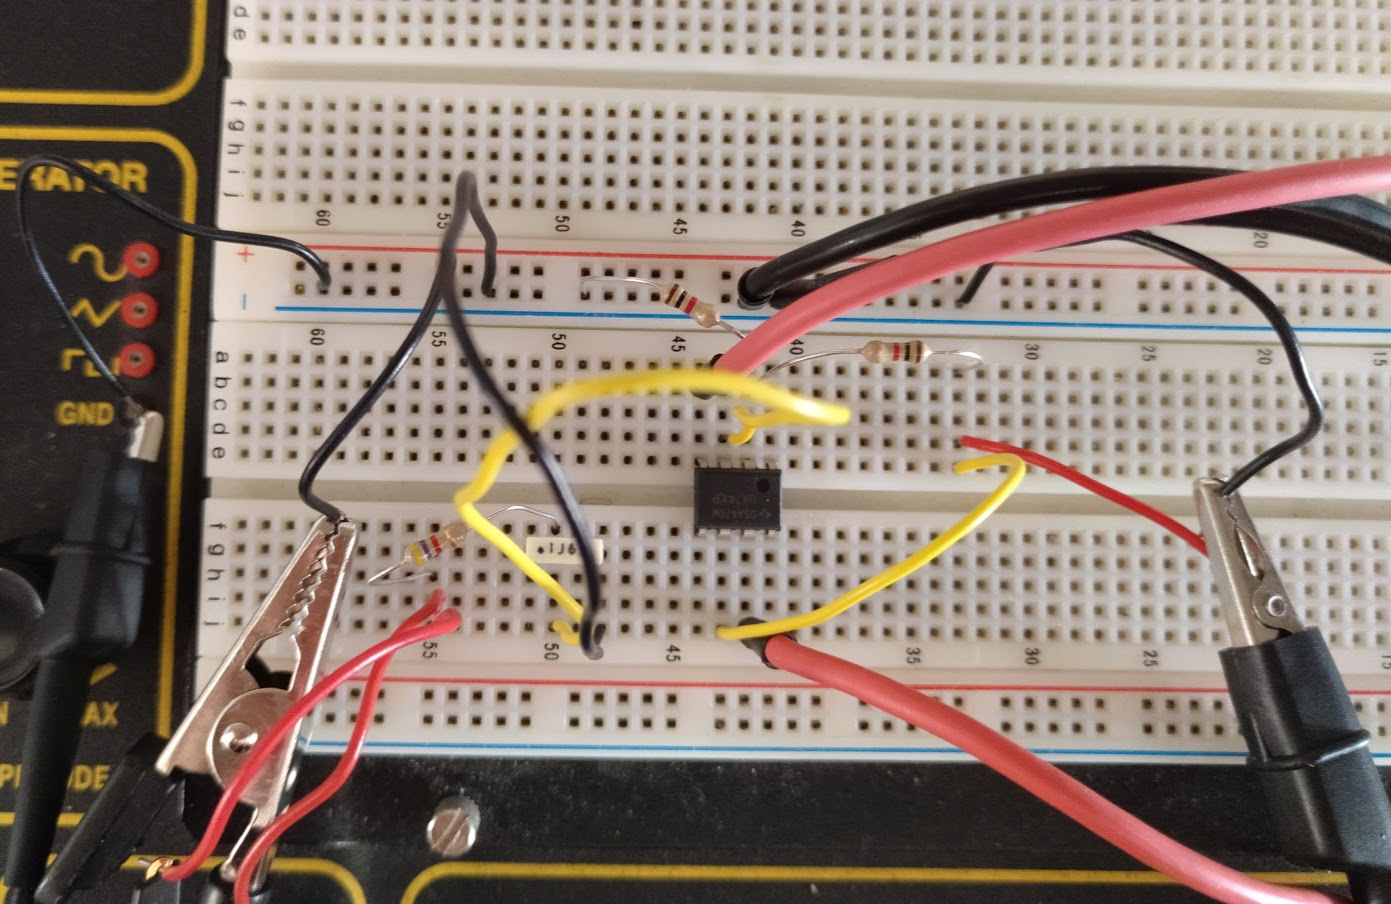
\includegraphics[scale=0.25]{circuito_img}\\
Circuito montado en la entrenadora.
\end{center}

\textbf{Varíe la frecuencia de la señal de entrada entre 80 Hz y 100 KHz. Mida la amplitud de
VL, la amplitud de V3 y el desfase entre VL y V3.}

\begin{center}
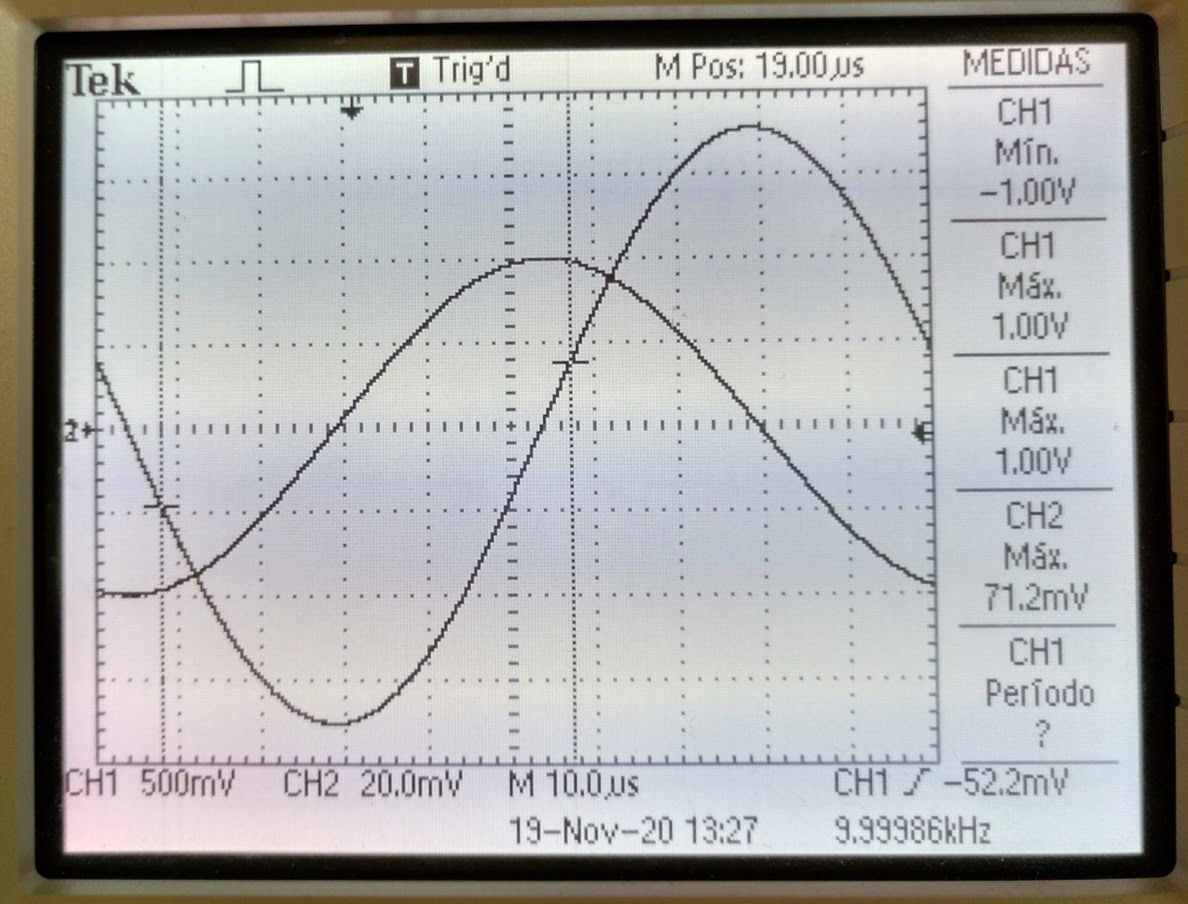
\includegraphics[scale=0.18]{ejemplo_A} 
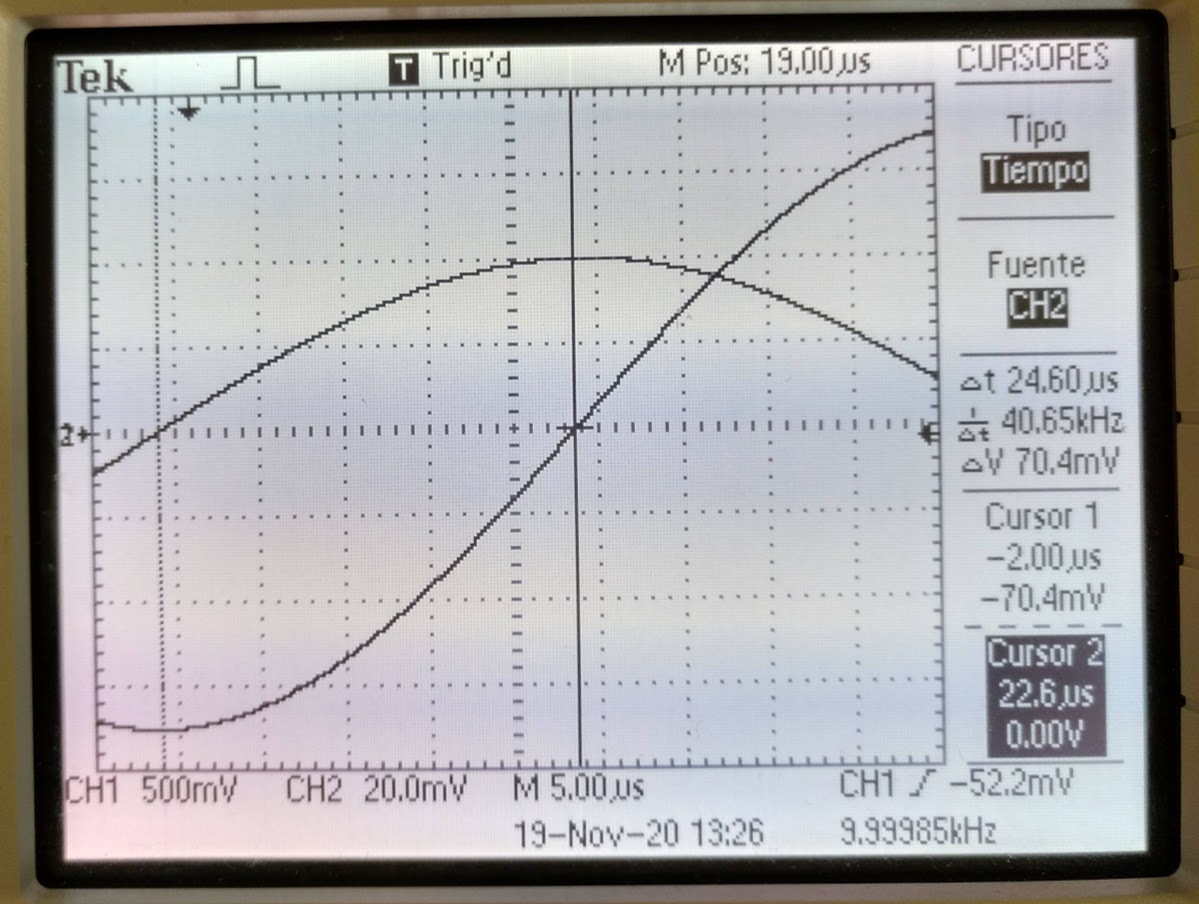
\includegraphics[scale=0.18]{ejemplo_t}\\
Ejemplo de la medición del valor Pico-Pico de las ondas (izquierda), y del desfase temporal con los cursores (derecha) en el osciloscopio.
\end{center}
 
\cleardoublepage

Tabla de los valores tomados:

\begin{table}[h!]
\centering
\begin{tabular}{|r|r|r|r|r|r|}
\hline
\multicolumn{1}{|l|}{frecuencia (Hz)} & \multicolumn{1}{l|}{$|V_L| (V)$} & \multicolumn{1}{l|}{$|V_3|(V)$} & \multicolumn{1}{l|}{$|A_v|=|V_L |/|V_3|$} & \multicolumn{1}{l|}{$\delta t(s)$} & \multicolumn{1}{l|}{$\Phi (^o)$} \\ \hline
80                                   & 2                              & 1 & 2               & 0,00048                            & -13,824     \\ \hline
100                                  & 1,96                           & 1,04                          & 1,884615385                & 0,00044                            & -15,84      \\ \hline
300                                  & 1,56                           & 1,04                          & 1,5                        & 0,00036                            & -38,88      \\ \hline
362                                  & 1,4 & 1 & 1,4                        & 0,00034                      & -44,3088      \\ \hline
500                                  & 1,16                           & 1,04                          & 1,115384615                & 0,000308                           & -55,44      \\ \hline
700                                  & 0,92                           & 1,04                          & 0,8846153846               & 0,00026                            & -65,52      \\ \hline
900                                  & 0,73                           & 1,04                          & 0,7019230769               & 0,00021                            & -68,04      \\ \hline
1000                                 & 0,672                          & 1,04                          & 0,6461538462               & 0,000192                           & -69,12      \\ \hline
3000                                 & 0,256                          & 1,04                          & 0,2461538462               & 0,000075                           & -81         \\ \hline
5000                                 & 0,14                           & 1,02                          & 0,137254902                & 0,0000472                          & -84,96      \\ \hline
7000                                 & 0,1                            & 1,02                          & 0,09803921569              & 0,0000352                          & -88,704     \\ \hline
9000                                 & 0,078                          & 1,02                          & 0,07647058824              & 0,000027                           & -87,48      \\ \hline
10000                                & 0,0712                         & 1                             & 0,0712                     & 0,0000246                          & -88,56      \\ \hline
30000                                & 0,0248                         & 1                             & 0,0248                     & 0,0000085                          & -91,8       \\ \hline
50000                                & 0,0152                         & 1,02                          & 0,01490196078              & 0,0000052                          & -93,6       \\ \hline
70000                                & 0,012                          & 1,02                          & 0,01176470588              & 0,0000037                          & -93,24      \\ \hline
90000                                & 0,0104                         & 1,04                          & 0,01                       & 0,00000286                         & -92,664    \\ \hline
100000                               & 0,0096                         & 1,02                          & 0,009411764706             & 0,00000256                         & -92,16    \\ \hline
\end{tabular}
\end{table}

Nota: se ha tomado también el valor de la ganancia para la frecuencia de valor f=362Hz, que es 1,40. Como se comenta en el apartado b), este valor se ha medido buscando la frecuencia de corte. Por otro lado, para el cálculo del desfase, se ha incluído el signo negativo que hace referencia al orden en el que se miden las señales en el osciloscopio (cuál aparece primero y cuál después) que, por los valores obtenidos en la simulación, sabemos que tienen que dar negativos.

\bigskip
\textbf{a) Represente los datos experimentales de ganancia (en dBs) y desfase en función de la
frecuencia usando una escala logarítmica para el de frecuencias. Compare los datos
experimentales con las curvas obtenidas de la simulación.}

Aquí se encuentra la gráfica de los valores experimentales de la ganancia de tensión en decibelios, comparada con las función teórica (calculada el trabajo previo).

\begin{center}
\includegraphics[scale=0.6]{gr_dB}\\
\end{center}

\cleardoublepage

Y la gráfica de la diferencia de fase entre $V_L$ y $V_{3}$, comparado con la función teórica.

\begin{center}
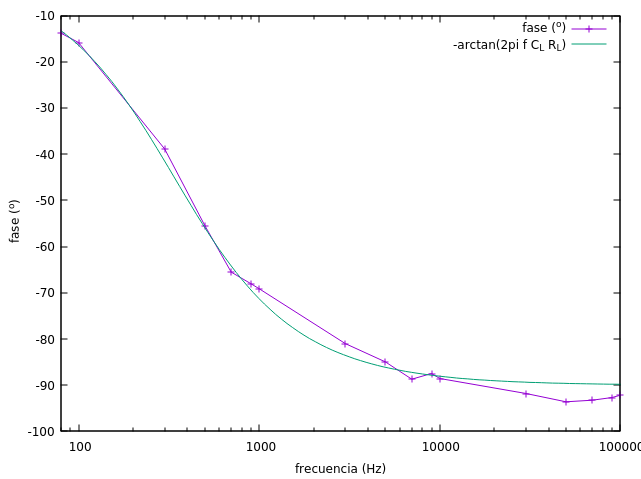
\includegraphics[scale=0.6]{fase}\\
\end{center}

Se puede apreciar en las gráficas que los datos medidos se ajustan muy bien a los teóricos. Aunque es cierto que las fases son más imprecisas por la dificultad que conlleva medir con precisión con los cursores del osciloscopio, que afecta bastante a las pequeñas desviaciones, porque es imposible en muchos casos medir exactamente el punto máximo de las ondas (o el punto de corte de estas con el eje x). Para ver mejor la proximidad de estos datos con los esperados, en la siguiente tabla incuyo una comparación entre algunos valores medidos en la simulación y los respectivos correspondientes al montaje experimental.

Nota: en la cuarta columna de esta tabla se encuentra el valor de la ganancia medida en LTSpice, no en decibelios, calculada de la siguiente forma: $|A_v|=10^{({|A_v|(dB)}/{20})}$. El error relativo ($E_r$, quinta columna) se ha calculado utilizando este valor y la ganancia experimental.

\begin{table}[h!]
\centering
\begin{tabular}{|r|r|r|r|r|r|r|r|}
\hline
\multicolumn{1}{|l|}{f (Hz)} & \multicolumn{1}{l|}{$|A_v|$} & \multicolumn{1}{l|}{$|A_v|$(LTS)(dB)} & \multicolumn{1}{l|}{$|A_v|$(LTS)} & \multicolumn{1}{l|}{$E_r(\%)$} & \multicolumn{1}{l|}{$\Phi (^o)$} & \multicolumn{1}{l|}{$\Phi (^o)$(LTS)} & \multicolumn{1}{l|}{LTS$\Phi-\Phi$} \\ \hline
100                                  & 1,884615385                  & 5,65                                                           & 1,916461063                                                & 1,66                    & -15,84                           & -16,49                                    & -0,65                 \\ \hline
300                                  & 1,5                          & 3,5156111                                                      & 1,49892725                                                 & 0,07                  & -38,88                           & -41,46                                    & -2,58                 \\ \hline
500                                  & 1,115384615                  & 0,991                                                          & 1,120856462                                                & 0,48                   & -55,44                           & -55,91                                    & -0,47                 \\ \hline
700                                  & 0,8846153846                 & -1,21                                                          & 0,8699614331                                               & 1,68                   & -65,52                           & -64,21                                    & 1,31                  \\ \hline
1000                                 & 0,6461538462                 & -3,86                                                          & 0,6412095766                                               & 0,77                    & -69,12                           & -71,3                                     & -2,18                 \\ \hline
3000                                 & 0,2461538462                 & -12,98                                                         & 0,2243881924                                               & 9,70                    & -81                              & -83,59                                    & -2,59                 \\ \hline
5000                                 & 0,137254902                  & -17,36                                                         & 0,1355189412                                               & 1,28                    & -84,96                           & -86,17                                    & -1,21                 \\ \hline
7000                                 & 0,09803921569                & -20,28                                                         & 0,09682778563                                              & 1,25                    & -88,704                          & -87,3                                     & 1,404                 \\ \hline
10000                                & 0,0712                       & -23,39                                                         & 0,06768617929                                              & 5,19                    & -88,56                           & -88,18                                    & 0,38                  \\ \hline
30000                                & 0,0248                       & -32,81                                                         & 0,02288231712                                              & 8,38                     & -91,8                            & -89,69                                    & 2,11                  \\ \hline
50000                                & 0,01490196078                & -37,37                                                         & 0,01353630091                                  & 10,09                    & -93,6                            & -90,19                                    & 3,41                  \\ \hline
70000                                & 0,01176470588                & -40,3                                                          & 0,00966050879                                              & 21,78                    & -93,24                           & -90,53                                    & 2,71                  \\ \hline
90000                                & 0,01                         & -42,45                                                         & 0,007542233958                                             & 32,58                    & -92,664                          & -90,82                                    & 1,844                 \\ \hline
100000                               & 0,009411764706               & -43,39                                                         & 0,006768617929                                             & 39,05                     & -92,16                           & -90,95                                    & 1,21                  \\ \hline
\end{tabular}
\end{table}

En esta tabla podemos ver que los valores experimentales de la ganancia son muy similares a los tomados en la simulación de LTSpice; aunque las ganancias tomadas con las frecuencias más altas, tienen un valor un poco mayor que el esperado, esto seguramente se deba a la precisión que tiene el osciloscopio al medir ondas con una ampitud tan baja (a partir de 50kHz se tiene un error mayor del $10\%$).

Las diferencias de fase entre las señales de entrada y salida tampoco difieren mucho de los datos esperados, no habiendo entre éstos y los medidos en el montaje más de 4$^o$ de diferencia (última columna de la tabla anterior).

\textbf{Fíjese que la onda de salida a altas frecuencias se vuelve triangular y que la amplitud decae. ¿A qué atribuye este comportamiento?}

En este filtro, al ser de paso bajo, en las frecuencias altas, las ganancias son muy bajas, por lo que las ondas están muy aplanadas y no se aprecia nada. Al menos en el caso de mi circuito, las ondas eran de apariencia sinusoidal en todos los casos, y tenían, como se ve en la tabla anterior, una amplitud mayor que la de la simulación.
\bigskip

\textbf{b) Determine la frecuencia de corte de forma experimental, busque el valor de frecuencia
para el cual, la ganancia se reduce a $1/2^{1/2}\approx 0,707$ de su valor máximo. Anote su valor
y el desfase entre la señal de entrada y la salida para esa frecuencia. Compare esta
frecuencia de corte con la calculada teóricamente y con la obtenida a partir de la
simulación con LTspice IV.}

La máxima ganancia calculada teóricamente es de valor 2 (medida para f=80Hz). Por tanto la ganancia de la frecuencia de corte tendrá un valor de $ \frac{2}{\sqrt2}\approx 1,414$, he buscado manualmente este valor, modificando la frecuencia, y he hallado que el valor que más se acercaba era para la frecuencia f=362Hz, con la que se tenía una ganancia de 1,40. El valor calculado teóricamente de la frecuencia de corte había sido (teniendo en cuenta los valores teóricos de la resistencia y el condensador): $f_c=338,628Hz$, por lo que en la medida experimental hemos tenido un error relativo de: 
$$E_{r}=100\times \frac{|338,628-362|}{338,628}=6,90\%$$
Sin embargo, si tenemos en cuenta que la resistencia que hemos utilizado tenía un valor de $R'_L=4,66k\Omega$, en lugar del valor con el que se calculó teóricamente esta frecuencia de corte, tenemos que la frecuencia de corte esperada es: 
$$ f'_c=\frac{1}{2\pi C_L R'_L}\approx341,53Hz$$ 
con la cual se calcula un error relativo de: 
$$E'_{r}=100\times \frac{|341,53-362|}{341,53}=5,99\%$$

El desfase medido con esta frecuencia es de -44,3088$^o$, que difiere en menos de 1$^o$ de la esperada para la frecuencia de corte: -45$^o$.
\bigskip

\textbf{c) Una vez obtenido un tono limpio y claro a la salida, incremente la frecuencia de la
señal de entrada hasta dejar de escuchar el tono asociado y anote el valor de frecuencia
(el valor más alto audible). Disminuya la frecuencia de la señal de entrada hasta dejar
de escuchar el tono asociado y anote el valor de frecuencia (el valor más bajo audible).}

No ha sido necesario conectar el condensador como se sugiere en caso de escuchar mucho ruido. Para todas las frecuencias audibles se escuchaba un tono claro.

El valor de frecuencia más alto audible ha sido de 17,2kHz. Sin embargo, en el caso de mi circuito, por mucho que bajara el valor de la frecuencia, siempre se escuchaba algo, para frecuencias de valores 50Hz, 30Hz, 20Hz, etc. se escuchaba el pitido muy grave y, según se bajaba más, se empezaban a apreciar los pulsos: a 1Hz se escuchaba con claridad un pulso por segundo, a 2Hz, dos pulsos por segundo, etc. Por tanto no había una frecuencia de la señal de entrada con la que, por abajo, se dejara de escuchar un tono asociado, aunque por supuesto, el cerebro humano no asocia los pulsos a tan bajas frecuencias a tonos, como sí hace con frecuencias más altas de 20Hz, por lo que se distinguían los pulsos por separado.

\end{document}